
\documentclass{report}

\usepackage[utf8]{inputenc}
\usepackage[italian]{babel}
\usepackage{import}
\usepackage{todonotes}
\usepackage{color}
\usepackage{rotating}
\usepackage[hidelinks]{hyperref}
\usepackage{url}
\usepackage{pdfpages}
\usepackage{siunitx}
\usepackage{pdflscape}
\usepackage{subfig}
\usepackage[euler]{textgreek}
\usepackage{mhchem}

\usepackage{multirow}

\usepackage{enumerate} 
\usepackage{amsmath}
\usepackage{amsfonts}

\usepackage[signatures,swapnames,sans]{frontespizio}

\usepackage{geometry}
\geometry{portrait, margin=3cm}
\usepackage{siunitx}
\usepackage{booktabs}

\renewcommand*\figurename{Figura}

\newcommand{\sub}[1]{\textsubscript{#1}}
\newcommand{\super}[1]{\textsuperscript{#1}}
\newcommand{\parallelsum}{\mathbin{\!/\mkern-5mu/\!}}

\newcommand{\Fig}[0]{Fig.}

\usepackage{titlesec}

\titleformat{\chapter}{\normalfont\huge}{}{20pt}{\huge\bfseries}

\linespread{1.3}


%% COMANDI UTILI
%\begin{table}[h]
%	\centering
%	\begin{tabular}{|c|c|c|}
%	\cline{2-3} 
%	\multicolumn{1}{c|}{} & \textbf{Valore nominale} & \textbf{Valore misurato}\\ 
%		%\hline
%		%{} & \textbf{Valore nominale} & \textbf{Valore misurato} \\ 
%		\hline
%		$\mathbf{R_1}$ & \SI{18}{k\ohm} & \SI{17.977}{k\ohm} \\ 
%		\hline
%		$\mathbf{R_2}$& \SI{1.8}{k\ohm} & \SI{1.815}{k\ohm} \\ 
%		\hline
%	\end{tabular}
%\caption{Misure delle resistenze utilizzate per il circuito.}
%\label{table:mis_res}
%\end{table}
%\begin{figure}[h!]
%\centering
%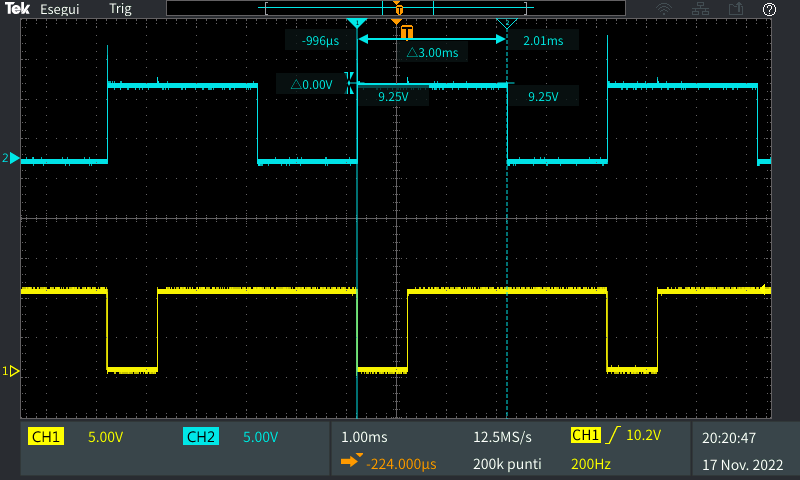
\includegraphics[height=6.5cm]{immagini/TEK00018}\\(a)\\[1ex]
%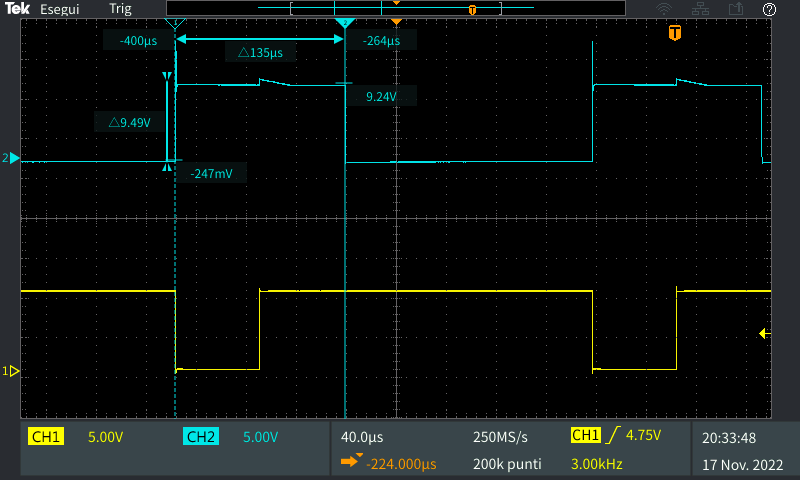
\includegraphics[height=6.5cm]{immagini/TEK00019}\\(b)
%\caption{Risposta del circuito con accoppiamento DC (a) e accoppiamento AC (b).}
%	\label{figura:accopp}
%\end{figure}

\begin{document}
\addtocounter{chapter}{+3}
	\begin{frontespizio}
		\Margini{3cm}{3cm}{3cm}{3cm}
		\Universita{Bergamo}
		\Logo[43.332mm]{unibg-mark}
		\Divisione{Scuola di Ingegneria}
		\Corso[Laurea Magistrale]{Ingegneria Informatica}
		\Titolo{Laboratorio di Elettronica}
		\Sottotitolo{Relazione esperienza di laboratorio 4}
		\Punteggiatura{}
		\NRelatore{Prof.}{Prof.}
		\Relatore{Luigi Gaioni}
		\Candidato[1058231]{Giulia Allievi}
		\Candidato[1059640]{Martina Fanton}
		\Annoaccademico{2022--2023}
		\begin{Preambolo*}
			\usepackage[italian]{babel}
			\usepackage[T1]{fontenc}
			\usepackage[utf8]{inputenc}
			\usepackage{microtype}
			\usepackage{lmodern}
			\graphicspath{{img/}}
			
			\renewcommand{\frontinstitutionfont}{\fontsize{14}{17}\bfseries\scshape}
			\renewcommand{\fronttitlefont}{\fontsize{17}{21}\bfseries\scshape}
			\renewcommand{\frontfootfont}{\fontsize{12}{14}\bfseries\scshape}
		\end{Preambolo*}
	\end{frontespizio}

%----------------------------------------------------------------------------------------
%	PAGINA BIANCA
%----------------------------------------------------------------------------------------
\newpage
\null
\thispagestyle{empty}
\newpage

%----------------------------------------------------------------------------------------
%	INTRO
%----------------------------------------------------------------------------------------
\chapter{Relazione attività di laboratorio 4}
\section*{Introduzione}
Nei circuiti analizzati durante questo laboratorio sono presenti diodi, amplificatori operazionali e un nuovo circuito integrato, il timer 555.\par
Nella figura \ref{figura:timer1} a sinistra, si può vedere la numerazione e la denominazione di ciascun pin di questo componente. Per capire quali sono i terminali, sul package è presente una mezza luna in corrispondenza del pin numero 1 e poi la numerazione prosegue in senso antiorario. Invece nella stessa figura a destra si possono notare i componenti interni di questo circuito integrato e in particolare della tipologia di timer LM555, ovvero quella che abbiamo utilizzato durante questo laboratorio.
\begin{figure}[h]
	\centering
	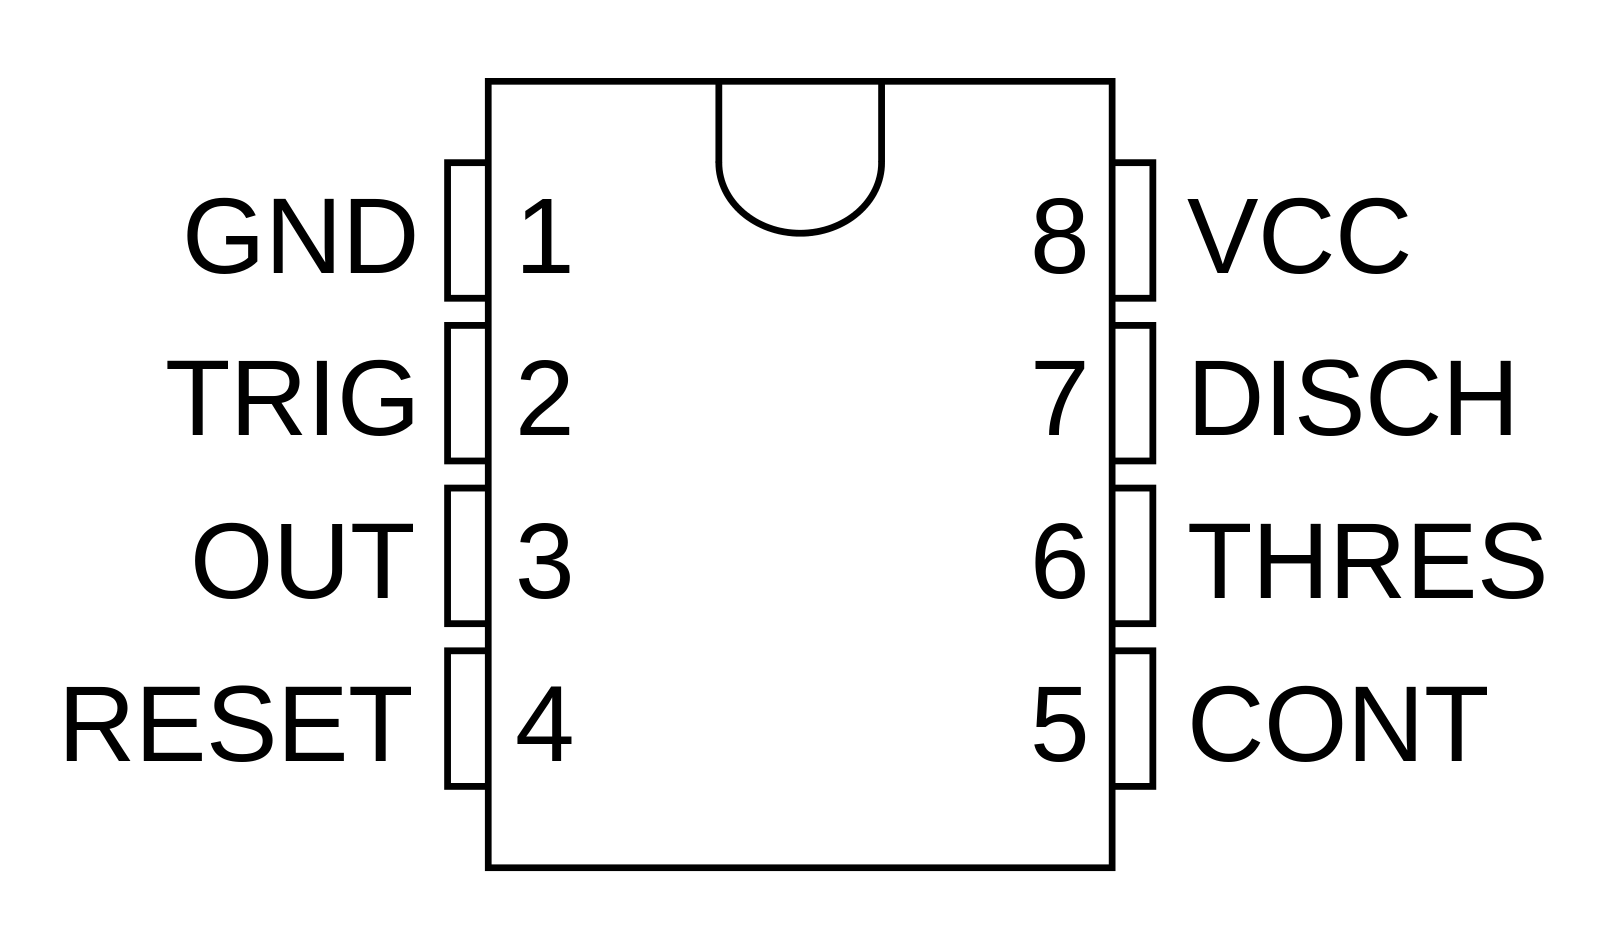
\includegraphics[height=4.6cm]{immagini/timer1}
	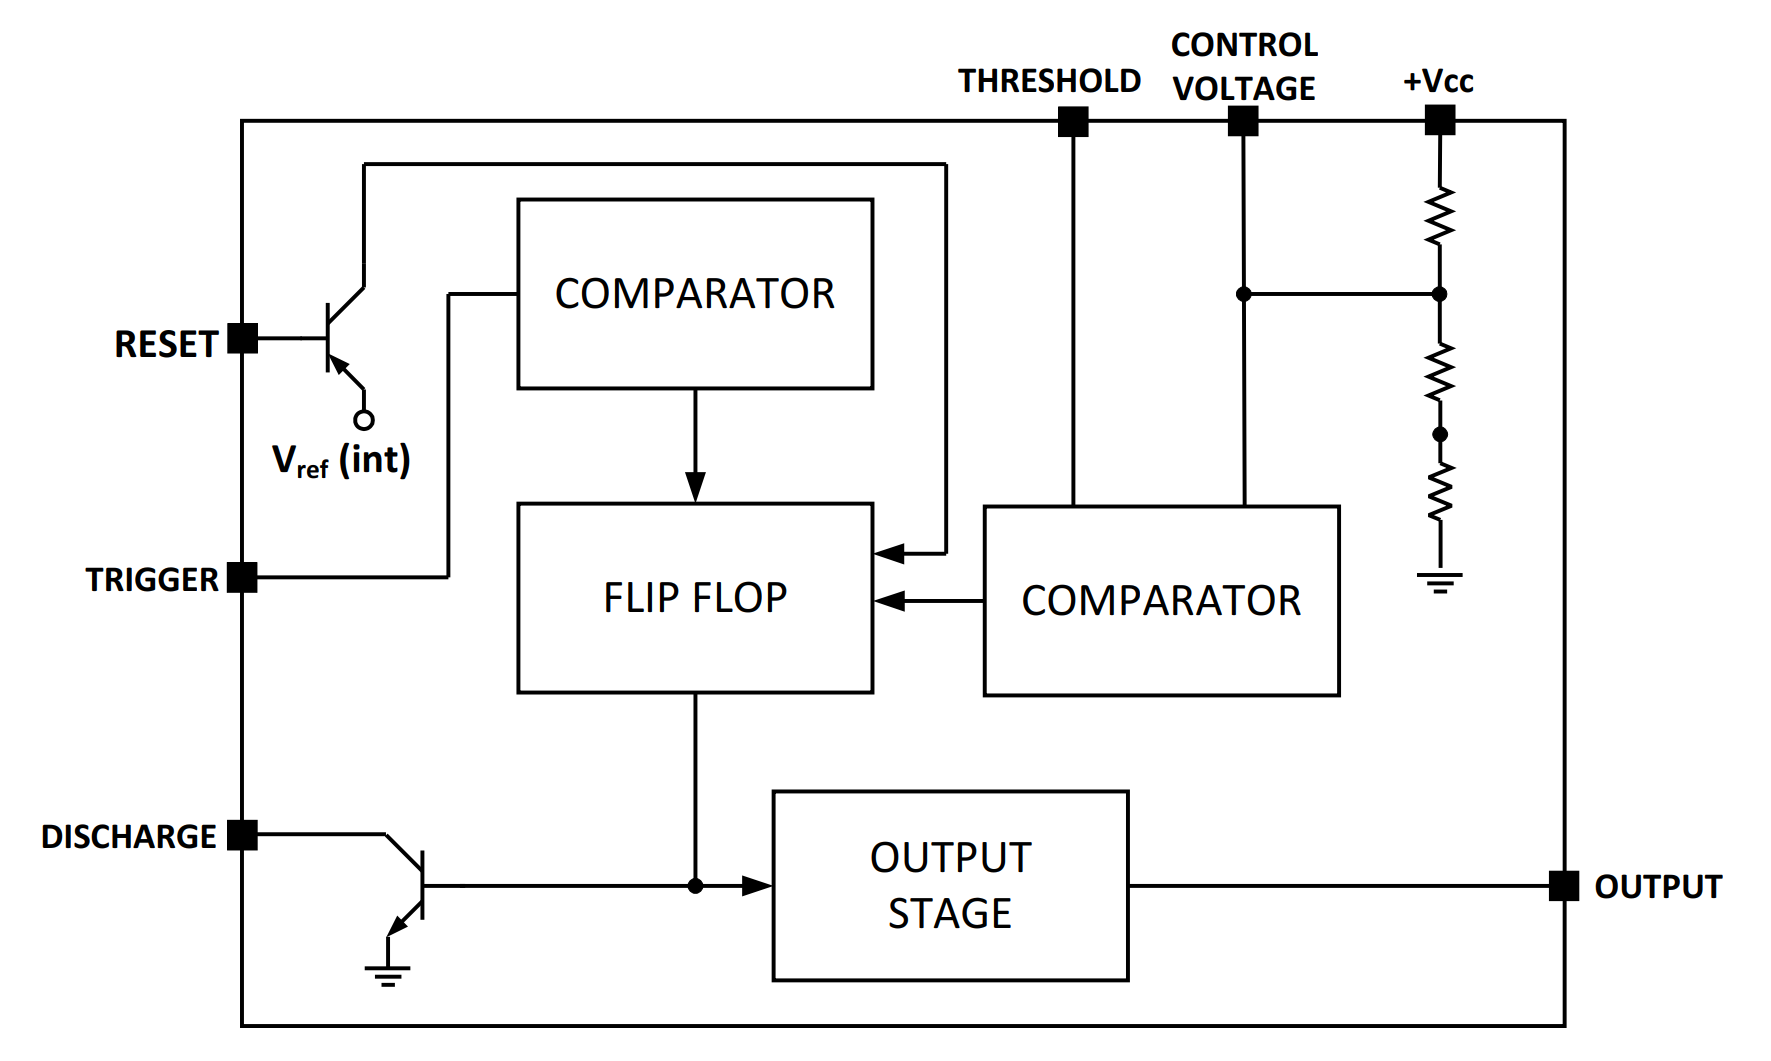
\includegraphics[height=4.6cm]{immagini/timer2}
	\caption{Package (a sinistra) e contenuto (a destra, fonte: \textcolor{blue}{\underline{\href{https://www.ti.com/lit/ds/symlink/lm555.pdf?ts=1667144089940&ref_url=https\%253A\%252F\%252Fwww.ti.com\%252Fproduct\%252FLM555}{datasheet}}} del LM555) del timer 555.}
	\label{figura:timer1}
\end{figure}
\\Questo componente richiede un'alimentazione singola per poter funzionare correttamente: va collegata la tensione positiva $\mathrm{V_{CC}}$ al pin 8, mentre la massa al pin 1.\par
Il timer 555 può essere utilizzato in due configurazioni: astabile oppure monostabile. In questo laboratorio abbiamo utilizzato la seconda configurazione, che è rappresentata nella figura \ref{figura:timer2}.
\begin{figure}[h]
	\centering
	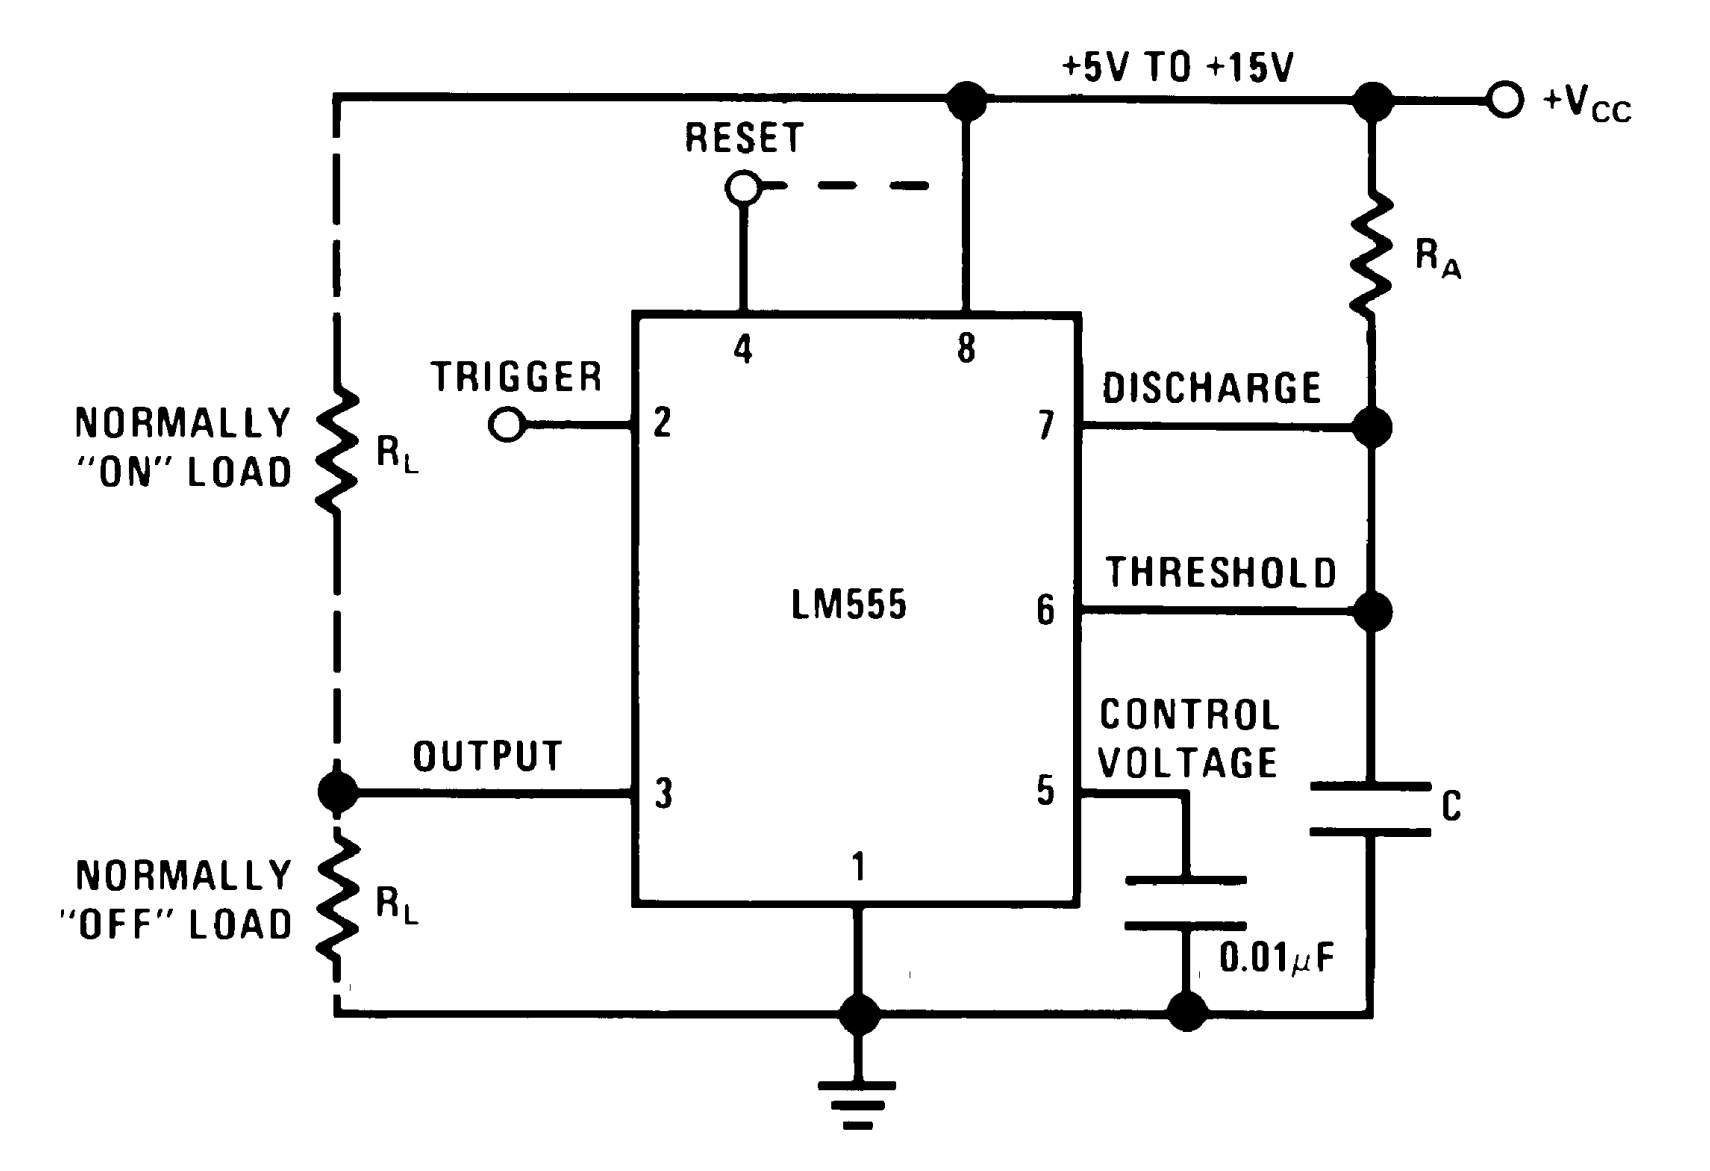
\includegraphics[height=4.6cm]{immagini/timer3}
	\caption{Configurazione monostabile del timer LM555 (fonte: \textcolor{blue}{\underline{\href{https://www.ti.com/lit/ds/symlink/lm555.pdf?ts=1667144089940&ref_url=https\%253A\%252F\%252Fwww.ti.com\%252Fproduct\%252FLM555}{datasheet}}} del LM555).}
	\label{figura:timer2}
\end{figure}

\newpage
\section{Circuito 1: circuito monostabile con trigger di Schmitt}
\subsection{Schema del circuito e Funzione di Trasferimento}
Questo circuito (in figura \ref{figura:schema1}) è stato ottenuto apportando delle modifiche all'oscillatore analizzato nel precedente laboratorio. In particolare sono stati aggiunti un diodo (con il catodo collegato a massa e con l'anodo collegato alla reazione negativa) e una rete di filtraggio (situata all'ingresso non invertente dell'amplificatore e collegata al circuito tramite un ulteriore diodo). Entrambi i diodi utilizzati sono di tipo 1N4148.\par
Per riuscire a visualizzare i segnali sull'oscilloscopio, abbiamo sostituito l'amplificatore \textmu A741 utilizzato nei precedenti laboratori con un OPAMP di tipo TL071, perché abbiamo osservato sperimentalmente che era più performante per questo particolare circuito.
\begin{figure}[h]
	\centering
	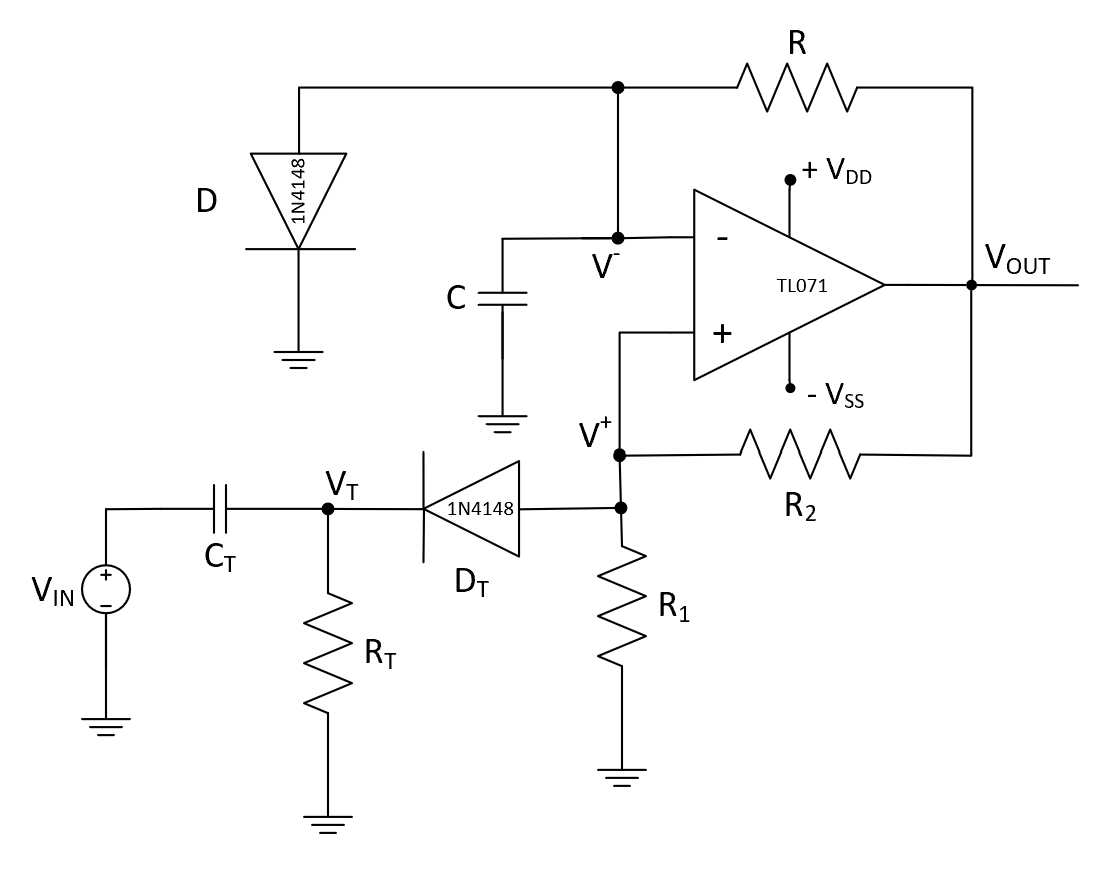
\includegraphics[height=7.5cm]{immagini/schema1}
	\caption{Schema del circuito monostabile con trigger di Schmitt.}
	\label{figura:schema1}
\end{figure}
\\\` E un circuito \textit{monostabile} perché presenta uno stato stabile, ovvero quello in cui la tensione di uscita $\displaystyle\mathrm{V_{OUT}}$ si trova a un valore pari a $\displaystyle\mathrm{V_{DD}}$ e dunque è possibile generare un impulso negativo fino a $\displaystyle\mathrm{V_{SS}}$ con una durata definita. Questa durata dipende dal processo di \todo{scarica?}{carica} del condensatore verso il valore di $\displaystyle\mathrm{V_{SS}}$ e questo processo viene interrotto quando viene raggiunta la soglia $\displaystyle\mathrm{V_L^+}$. Difatti la tensione sul condensatore può essere calcolata come:
\\[2pt]\indent$\displaystyle{\mathrm{V_C(t)}=\mathrm{V^-(t)}=\mathrm{V_{SS}}+(0.7-\mathrm{V_{SS}}) \cdot e^{-\frac{t-t_0}{\tau}}}$
\\dove $\mathrm{t_0}$ è l'istante in cui si ha il fronte di discesa del segnale in ingresso $\mathrm{V_{IN}}$ e l'inizio del processo di carica del condensatore verso il valore $\mathrm{V_{SS}}$, mentre $\mathrm{\tau}$ corrisponde alla costante di tempo data da: \\\indent$\displaystyle{\mathrm{\tau}= R \cdot C}$.
\\Da questa equazione si può ricavare la formula della durata dell'impulso negativo in uscita:
\\[2pt]\indent$\displaystyle{T_A=\tau\cdot\ln\biggl(1+\frac{R_2}{R_1}\biggr)\indent \mathrm{se\;}|V_{SS}|\gg\SI{0.7}{\volt}}$
\subsection{Analisi e dati sperimentali}
Per poter costruire il circuito sulla breadboard, per prima cosa sono stati scelti i valori dei componenti da utilizzare. Nel caso delle resistenze, le loro misure sono state riportate nella tabella \ref{table:mis_res1}, mentre per i condensatori sono state utilizzate delle capacità di valore nominale di \SI{150}{n\farad} per C e di \SI{1}{n\farad} per $\mathrm{C_T}$.
\begin{table}[h!]
	\centering
	\begin{tabular}{|c|c|c|}
		\cline{2-3} 
		\multicolumn{1}{c|}{} & \textbf{Valore nominale} & \textbf{Valore misurato}\\ 
		\hline
		$\mathbf{R}$ & \SI{12}{k\ohm} & \SI{11.882}{k\ohm} \\ 
		\hline
		$\mathbf{R_1}$ & \SI{12}{k\ohm} & \SI{11.934}{k\ohm} \\ 
		\hline
		$\mathbf{R_2}$ & \SI{12}{k\ohm} & \SI{11.950}{k\ohm} \\ 
		\hline
		$\mathbf{R_T}$ & \SI{12}{k\ohm} & \SI{11.894}{k\ohm} \\ 
		\hline
	\end{tabular}
	\caption{Misure delle resistenze utilizzate per il circuito.}
	\label{table:mis_res1}
\end{table}
\\Una volta costruito il circuito (figura \ref{figura:circuito1}), è stato alimentato con una tensione duale di $\mathrm{\pm\SI{10}{\volt}}$ e poi gli è stato fornito in ingresso un segnale a onda quadra (detto segnale di trigger) con duty cycle del 20\% e frequenza di \SI{100}{\hertz}.
\begin{figure}[h]
	\centering
	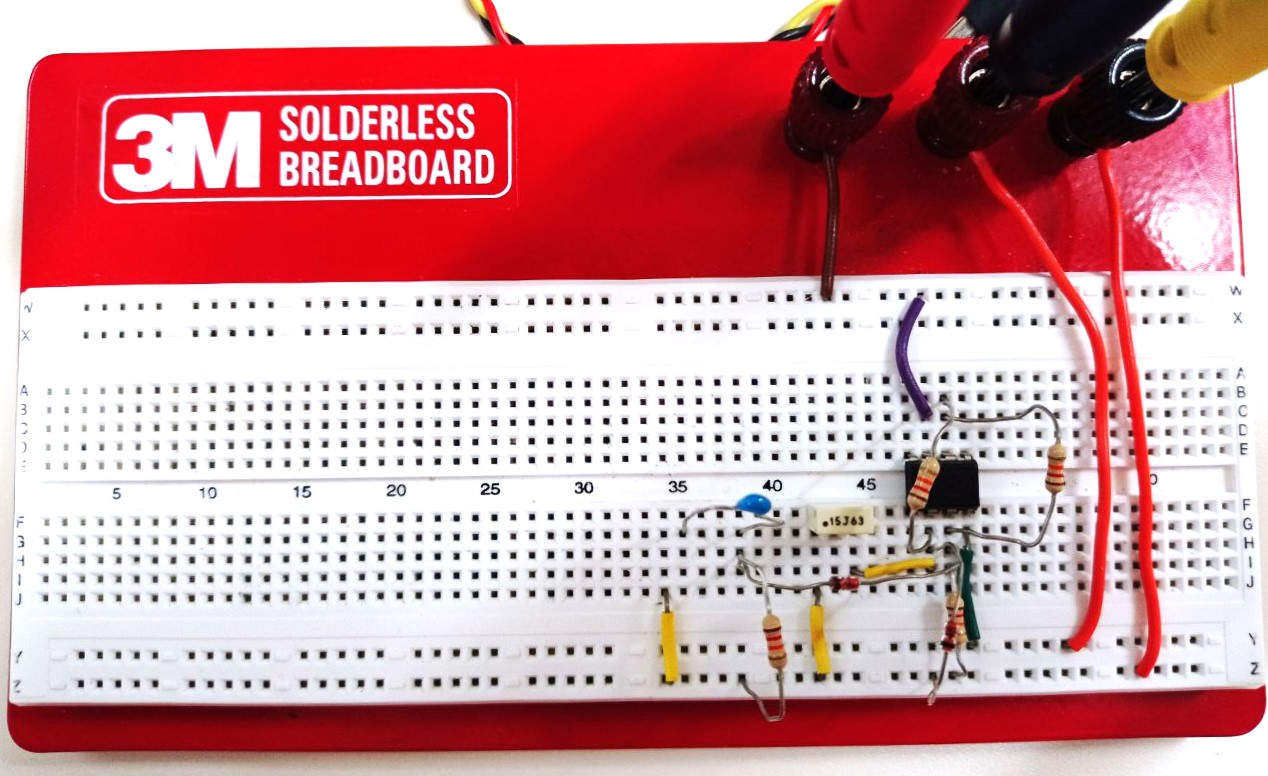
\includegraphics[height=6.5cm]{immagini/circuito1}
	\caption{Fotografia del circuito monostabile con trigger di Schmitt realizzato in laboratorio.}
	\label{figura:circuito1}
\end{figure}
\\\indent Nella figura \ref{figura:TEK00002} sono mostrati il segnale in ingresso $\mathrm{V_{IN}}$ (in giallo, CH1) e il segnale in uscita $\mathrm{V_{OUT}}$ (in azzurro, CH2).\par
Successivamente, abbiamo utilizzato le formule descritte nella sezione precedente per verificare la correttezza della misura della durata dell'impulso negativo in uscita ($\mathrm{T_A}$) ottenuta con l'oscilloscopio:
\\[4pt]\indent$\displaystyle{T_A=\tau\cdot\ln\biggl(1+\frac{R_2}{R_1}\biggr)=\SI{1.8}{m\second}\cdot\ln\biggl(1+\frac{\SI{12}{k\ohm}}{\SI{12}{k\ohm}}\biggr)=\SI{1.248}{m\second}}$
\\[4pt]\indent con $\displaystyle{\tau=R \cdot C=\SI{12}{k\ohm}\cdot\SI{150}{n\farad}=\SI{1.8}{m\second}}$
\\[4pt]La verifica è quindi soddisfatta perché l'oscilloscopio misura una durata dell'impulso di \SI{1.312}{m\second}, dunque l'errore tra i due valori è circa del 4\%. Questa percentuale di errore è causata in parte anche dall'imprecisione del valore del duty cycle dell'onda quadra in ingresso. In particolare questa imprecisione è dovuta all'errore della strumentazione utilizzata siccome sul generatore di forme d'onda è stato applicato un duty cycle pari al 20\% mentre l'oscilloscopio ne rileva un valore di 19.95\% (in figura \ref{figura:TEK00002}) e quindi leggermente inferiore. Di conseguenza la rilevazione sull'oscilloscopio di una durata dell'impulso negativo maggiore è determinata dal fatto che l'onda rimane a un livello basso per più tempo rispetto al periodo basso teorico.
\\Poi sono state confrontate la durata dell'impulso negativo in uscita $\mathrm{T_A}$ con la durata dell'impulso negativo in ingresso $\mathrm{T_B}$, calcolata come:
\\[4pt]\indent$\displaystyle{T_B=(1-\delta)\cdot T=(1-20\%)\cdot\SI{10}{m\second}=\SI{8}{m\second}}$
\\[4pt]\indent con f = \SI{100}{\hertz} $\Rightarrow\;\displaystyle{T=\frac{1}{f}=\SI{10}{m\second}}$
\\[4pt]Come ci si aspetta dalla teoria, si ottiene che $\mathrm{T_B}>>\mathrm{T_A}$.
\begin{figure}[h]
	\centering
	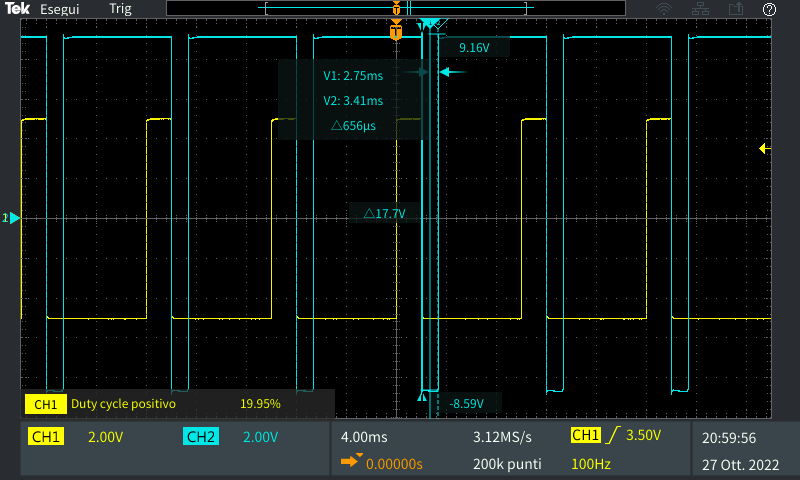
\includegraphics[height=5.5cm]{immagini/TEK00002}
	\caption{Confronto di $\mathrm{V_{IN}}$ (CH1) con $\mathrm{V_{OUT}}$ (CH2) con misure dell'oscilloscopio.}
	\label{figura:TEK00002}
\end{figure}
\\Inoltre sono stati anche confrontati i segnali delle tensioni in ingresso e in uscita rispetto a quelle presenti sugli ingressi dell'OPAMP e a quella presente nel nodo $\mathrm{V_T}$.
\begin{figure}[h]
	\centering
	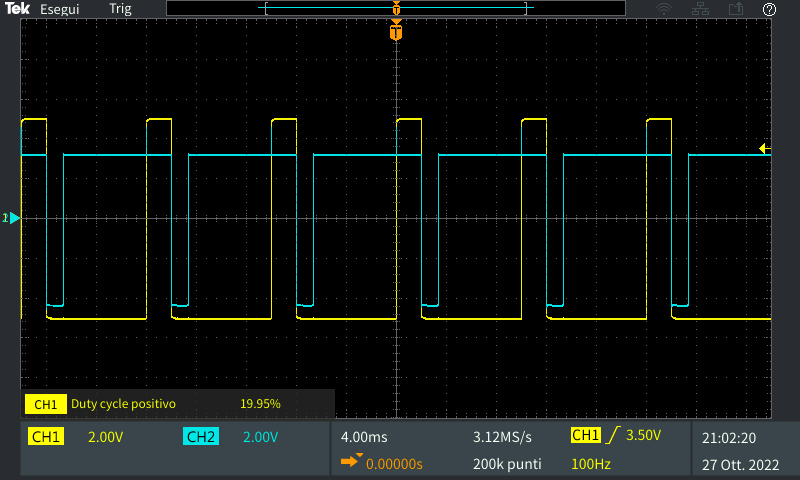
\includegraphics[height=6cm]{immagini/TEK00003}
	\caption{Confronto di $\mathrm{V_{IN}}$ (CH1) con $\mathrm{V^+}$ (CH2).}
	\label{figura:TEK00003}
\end{figure}
\begin{figure}[h]
	\centering
	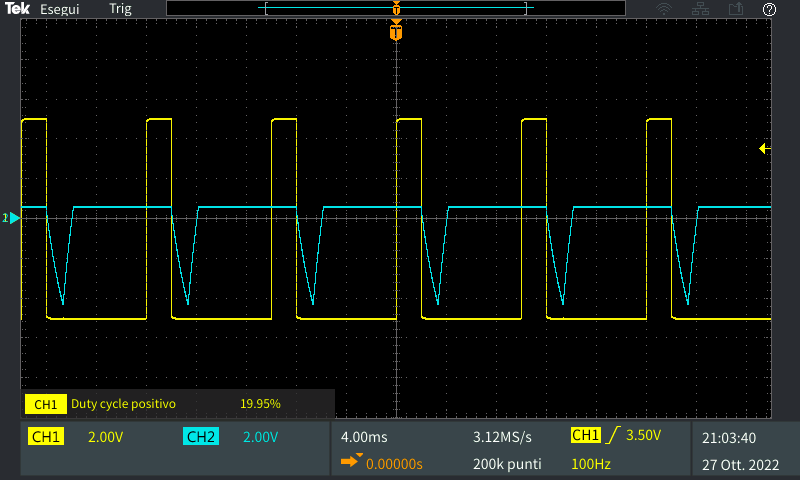
\includegraphics[height=4.6cm]{immagini/TEK00004}
	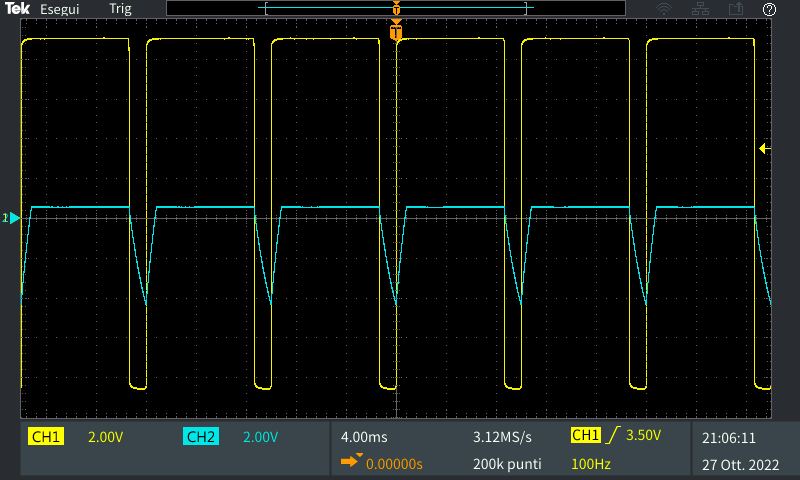
\includegraphics[height=4.6cm]{immagini/TEK00005}
	\caption{Confronto di $\mathrm{V^-}$ (CH2) con $\mathrm{V_{IN}}$ (CH1 a sinistra) e con $\mathrm{V_{OUT}}$ (CH1 a destra).}
	\label{figura:TEK00004e5}
\end{figure}
\\Per quanto riguarda la tensione sull'ingresso non invertente $\mathrm{V^+}$, essa varia tra $\mathrm{V_L^+}$ e $\mathrm{V_H^+}$ e, come si può notare dalla figura \ref{figura:TEK00003}, questi due valori non sono simmetrici. Questo succede perché:
\begin{itemize}
	\item se $\mathrm{V_{OUT}}$ è negativa (ovvero pari a $\mathrm{V_{SS}}$) si ha che il diodo $\mathrm{D_T}$ è spento e quindi:
	\\[4pt]$\displaystyle{\;\;\;V_L^+=\frac{V_{SS}}{2}=\frac{\SI{-10}{\volt}}{2}=\SI{-5}{\volt}}$;
	\item se $\mathrm{V_{OUT}}$ è positiva (ovvero pari a $\mathrm{V_{DD}}$) si ha che il diodo $\mathrm{D_T}$ è accesso e quindi:
	\\[4pt]$\displaystyle{\;\;\;V_H^+=\frac{V_{DD}}{3}=\frac{\SI{10}{\volt}}{3}=\SI{3.33}{\volt}}$.
\end{itemize}
Invece la tensione sull'ingresso invertente $\mathrm{V^-}$, corrispondente alla tensione sul condensatore C ($\mathrm{V_C}$), è stata rappresentata nella figura \ref{figura:TEK00004e5} e presenta un'espressione nel tempo pari a:
\\[4pt]\indent$\displaystyle{V_C(t)=V^-(t)=V_{SS}+(0.7-V_{SS})\cdot e^{-\frac{t-t_0}{\tau}}=\SI{-10}{\volt}+\SI{10.7}{\volt}\cdot e^{-\frac{t-t_0}{\SI{1.8}{m\second}}}}$
\\[4pt]TODO: METTERE VALORE DI t0 NELL'ESPRESSIONE DI V-
\\Infine considerando la tensione $\mathrm{V_T}$, TODO: FINIRE TESTO + MANCANO FOTO OSCILLOSCOPIO
\\TODO: MANCANO FOTO OSCILLOSCOPIO STATO STABILE

\newpage
\section{Circuito 2: circuito monostabile con NE555}
\subsection{Schema del circuito e Funzione di Trasferimento}
\begin{figure}[h]
	\centering
	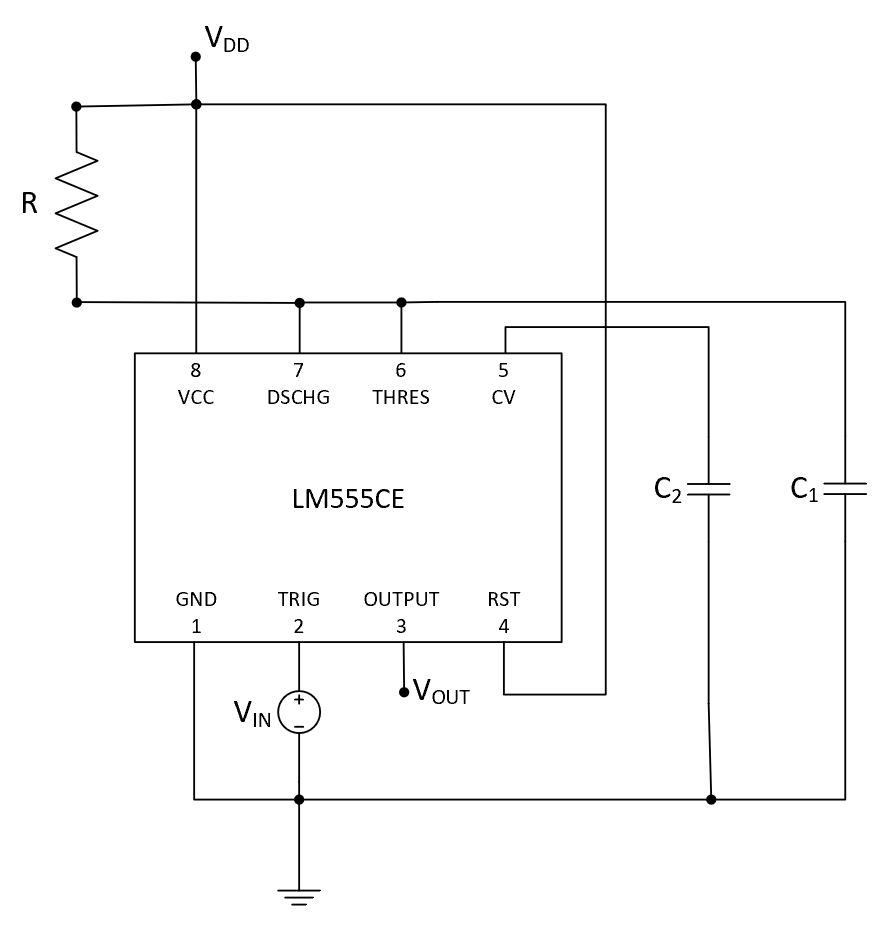
\includegraphics[height=7.5cm]{immagini/schema2}
	\caption{Schema del circuito monostabile con NE555.}
	\label{figura:schema2}
\end{figure}
\subsection{Analisi e dati sperimentali}
%R ... k\ohm --> 12k\ohm
%R 4.698 k\ohm --> 4.7 k\ohm
\begin{figure}[h]
	\centering
	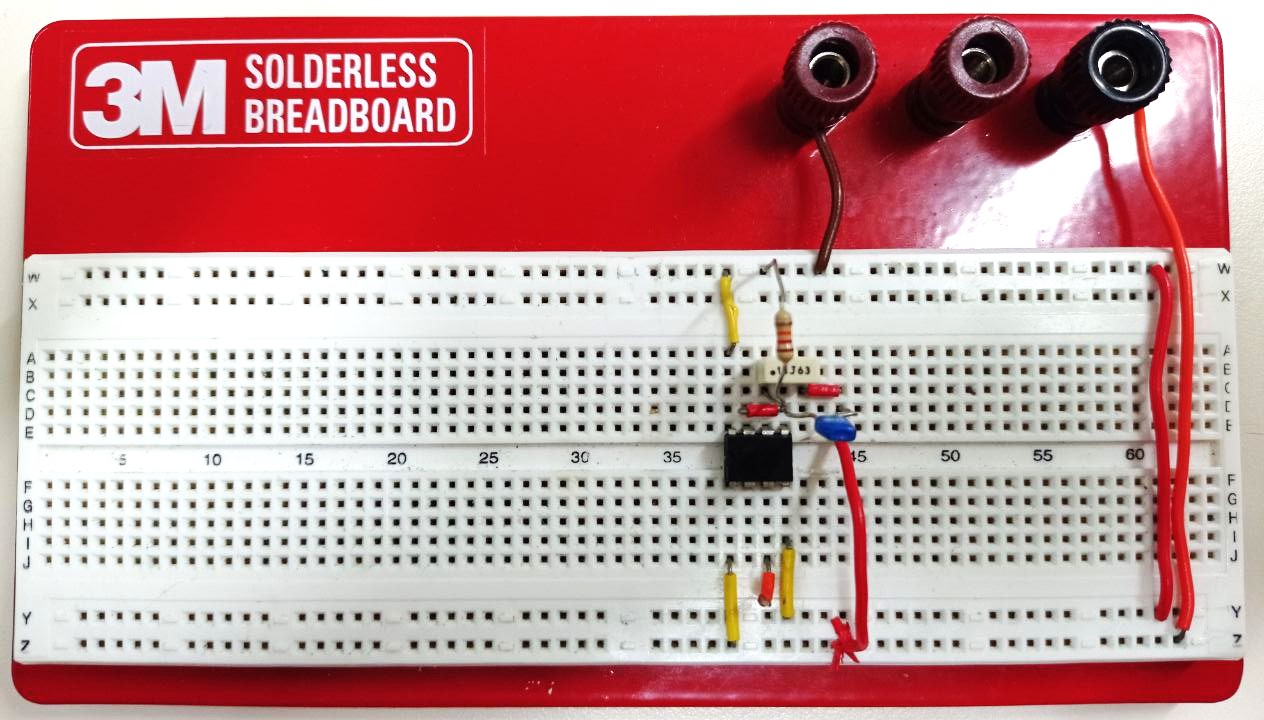
\includegraphics[height=6.5cm]{immagini/circuito2}
	\caption{Fotografia del circuito monostabile con LM555 realizzato in laboratorio.}
	\label{figura:circuito2}
\end{figure}

%----------------------------------------------------------------------------------------

\end{document}
